\documentclass{article}
\usepackage[utf8]{inputenc}
\usepackage[hmargin=2.5cm,vmargin=3cm,bindingoffset=0.5cm]{geometry}
\usepackage{graphicx}
\graphicspath{ {figures/} }
\usepackage{listings}
\usepackage{hyperref}
\renewcommand{\lstlistingname}{Auflistung}

\begin{document}

\pagenumbering{alph}
\begin{titlepage}
  \begin{center}
    
\includegraphics[width=\textwidth]{THD-Logo.pdf}
    \vspace{1cm}
    \rule{1\textwidth}{1mm} \\[0.3cm]
    \textsc{\scshape \huge Bachelor Cyber Security}\\
    \rule{1\textwidth}{1mm} \\[2cm]
    {
      \vspace{1cm}
      \Large \textbf{Kryptologie 2}
      \vspace{3cm}
      \Large \textbf{Projektbericht}
    }\\[0.5cm]
    \LARGE \textbf{Ausarbeitung Cryptochallenge: CurveBall}\\[2cm]
    \begin{minipage}[t]{0.4\textwidth}
      \begin{flushleft}
        \normalsize \emph{Autor:}\\[0.3cm]
        Manuel Friedl, Matrikel-Nr.: 1236626\\
        Christof Renner, Matrikel-Nr.: 22301943
      \end{flushleft}
    \end{minipage}
    \begin{minipage}[t]{0.5\textwidth}
      \begin{flushright}
        \normalsize \emph{Betreuer:}\\[0.3cm]
        Prof. Dr. Martin Schramm
      \end{flushright}
    \end{minipage}\\[3cm]
    {\large Deggendorf – \today\\}
  \end{center}
\end{titlepage}

\newpage
\pagenumbering{Roman}

\newpage
\tableofcontents
\newpage

\pagenumbering{arabic}

\section{Einleitung und Hintergrund}
CVE-2020-0601, bekannt als \textbf{CurveBall}, ist eine kritische Schwachstelle in der Windows CryptoAPI. Die Sicherheitslücke erlaubt Angreifern, gefälschte ECC-Zertifikate zu erzeugen, indem sie elliptische Kurvenparameter manipulieren, speziell den Generatorpunkt G.

\section{Projektübersicht und Zielsetzung}
Das Projekt 'SS25-Kryptologie2' bietet eine interaktive Web-basierte Simulation der CurveBall-Schwachstelle. Ziel ist es, diese Sicherheitslücke eigenständig zu simulieren, zu verstehen und praxisnah zu analysieren.

\section{Beschreibung der Webinterface-Simulation}
Das Webinterface ermöglicht eine intuitive Bedienung der Challenge, unterteilt in die folgenden Schritte:

\subsection{Aufbau und Übersicht}
Das Interface gliedert sich in drei zentrale Bereiche:

\begin{enumerate}
    \item Schlüsselgenerierung
    \item Zertifikatsgenerierung
    \item Validierungssimulation
\end{enumerate}

\begin{figure}[h]
\centering
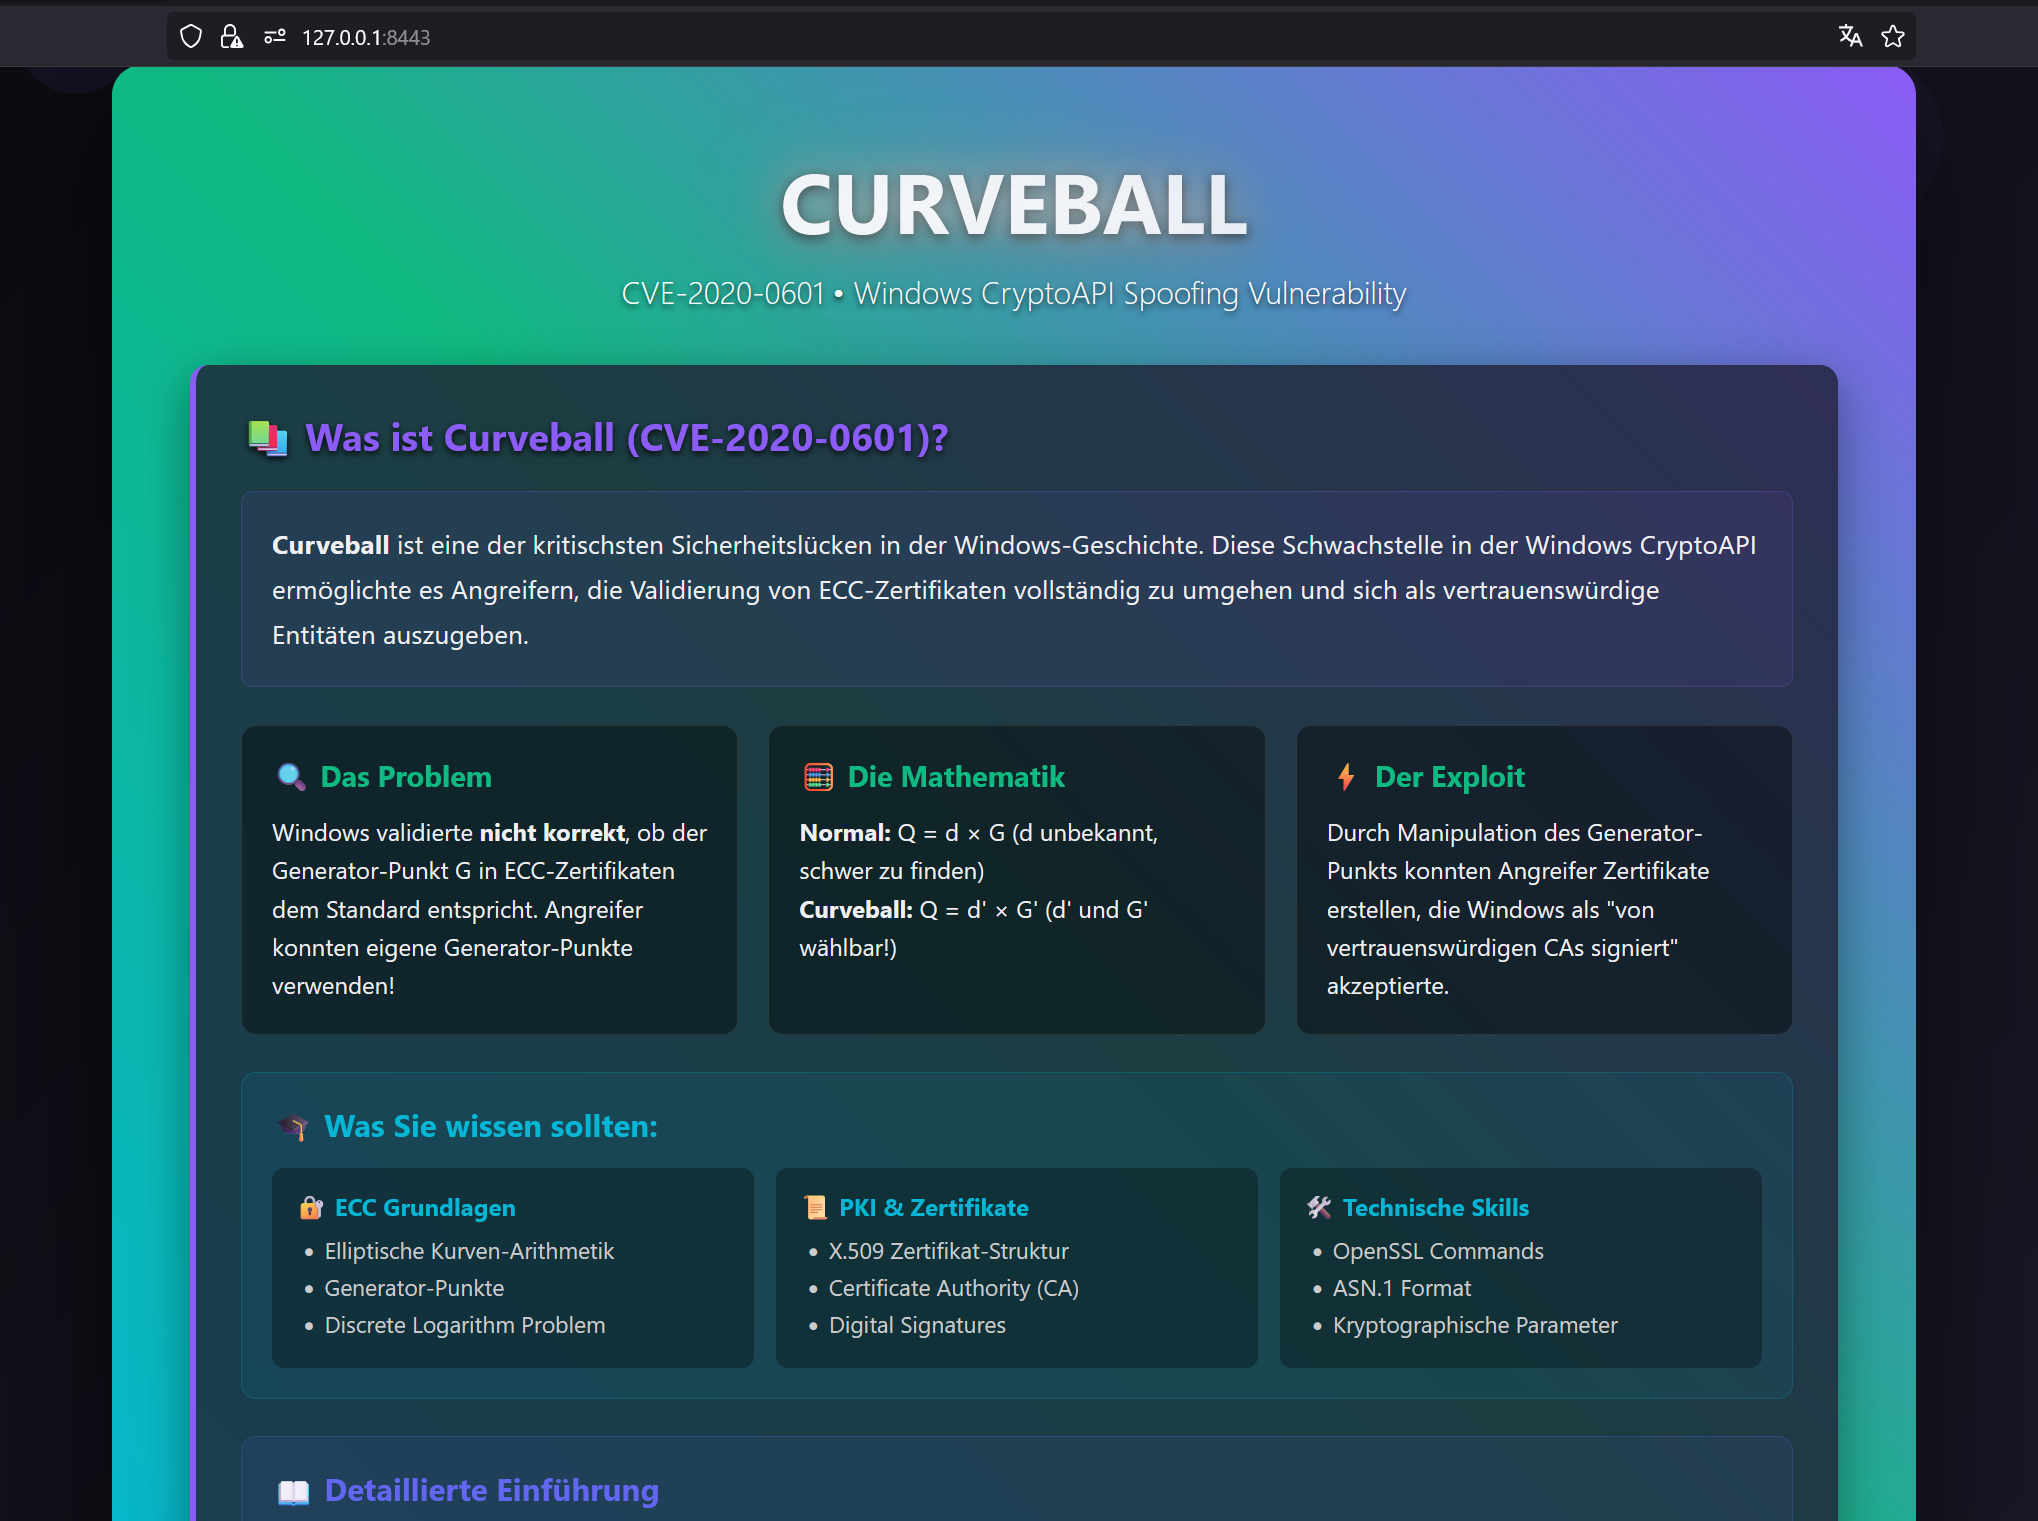
\includegraphics[width=0.9\textwidth]{webinterface_overview.png}
\caption{Übersicht des Webinterfaces (Platzhalter)}
\end{figure}

\subsection{Schlüsselgenerierung über das Webinterface}
Im ersten Schritt wird über die Oberfläche das Python-Skript \texttt{gen-key.py} ausgeführt, welches aus einem gültigen CA-Zertifikat einen manipulierten ECC-Schlüssel erzeugt.

\begin{lstlisting}[language=bash,caption={Schlüsselgenerierung}]
python gen-key.py USERTrustECCCertificationAuthority.crt
\end{lstlisting}

\begin{figure}[h]
\centering
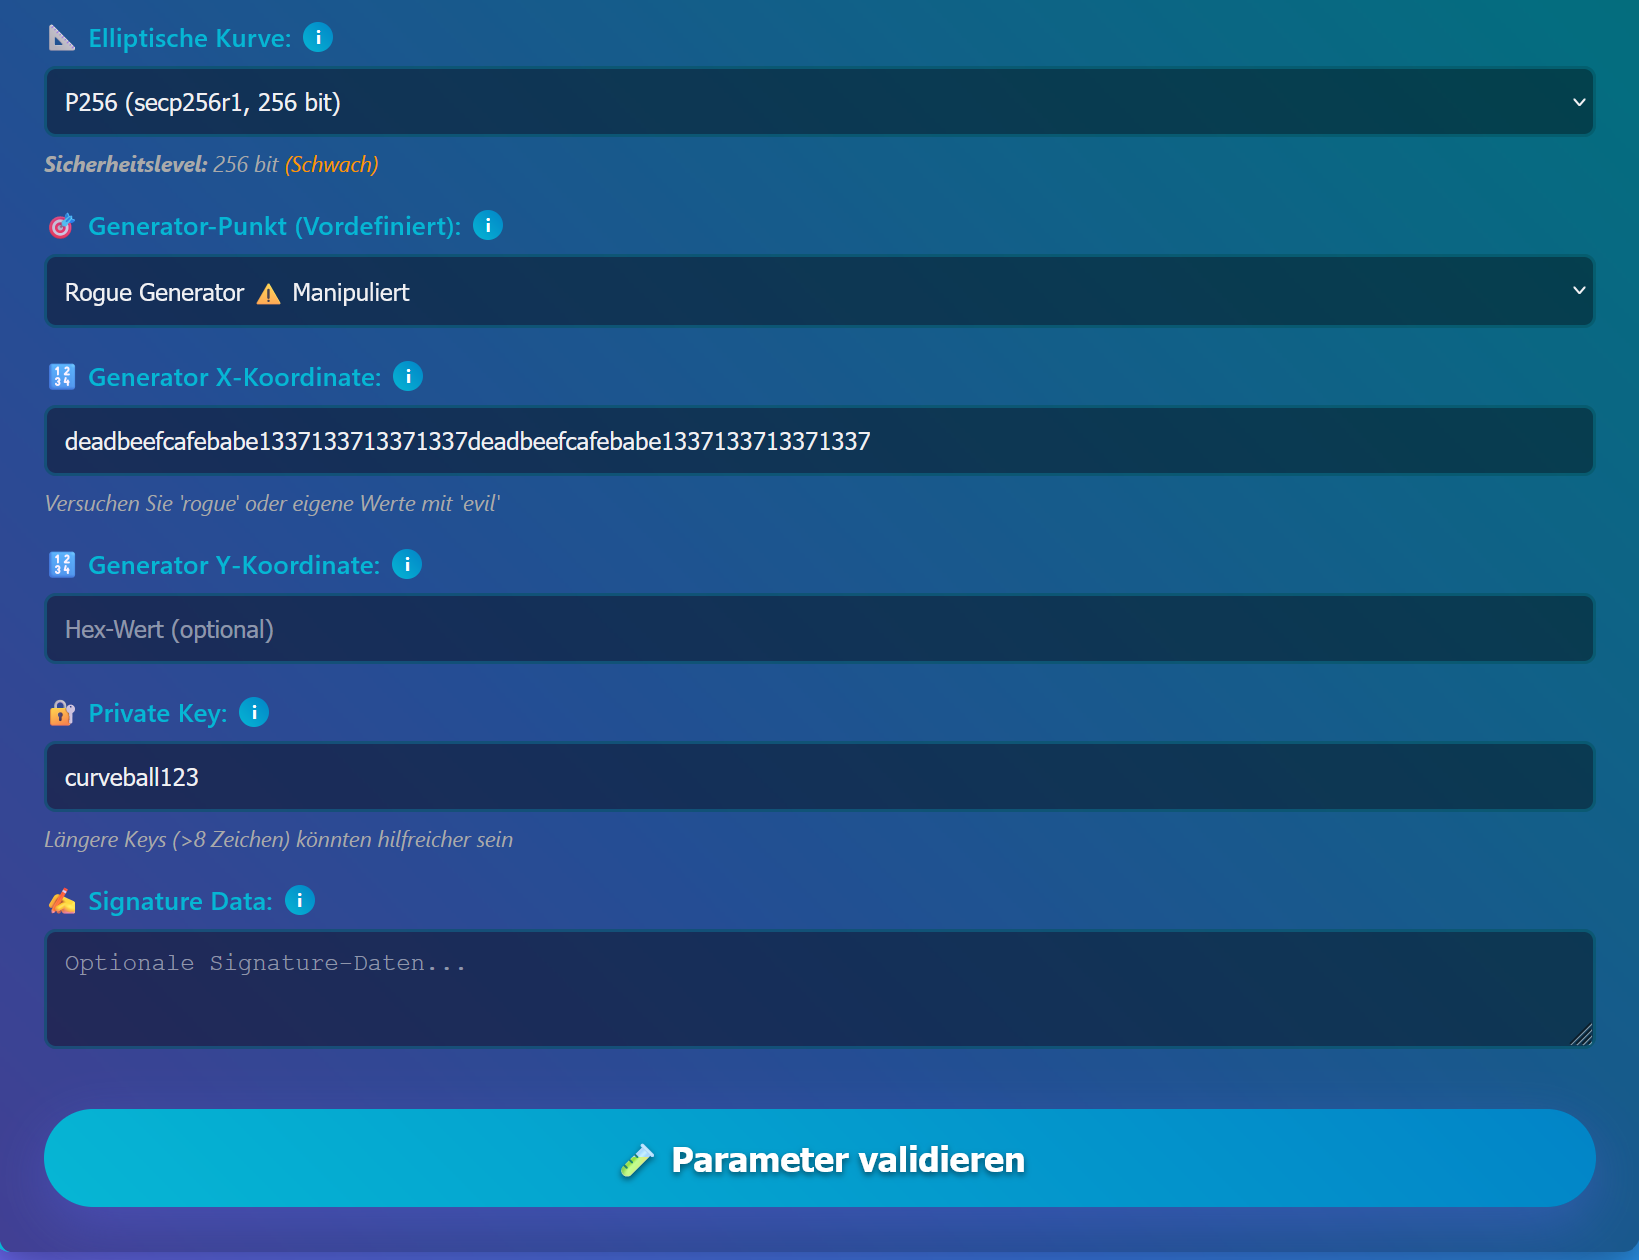
\includegraphics[width=0.8\textwidth]{webinterface_keygen.png}
\caption{Webinterface Schlüsselgenerierung}
\end{figure}

\subsection{Zertifikatsgenerierung}
Im nächsten Schritt erfolgt die automatische Zertifikatsgenerierung via OpenSSL mithilfe des generierten Schlüssels und vordefinierter Konfigurationsdateien.

\begin{figure}[h]
\centering
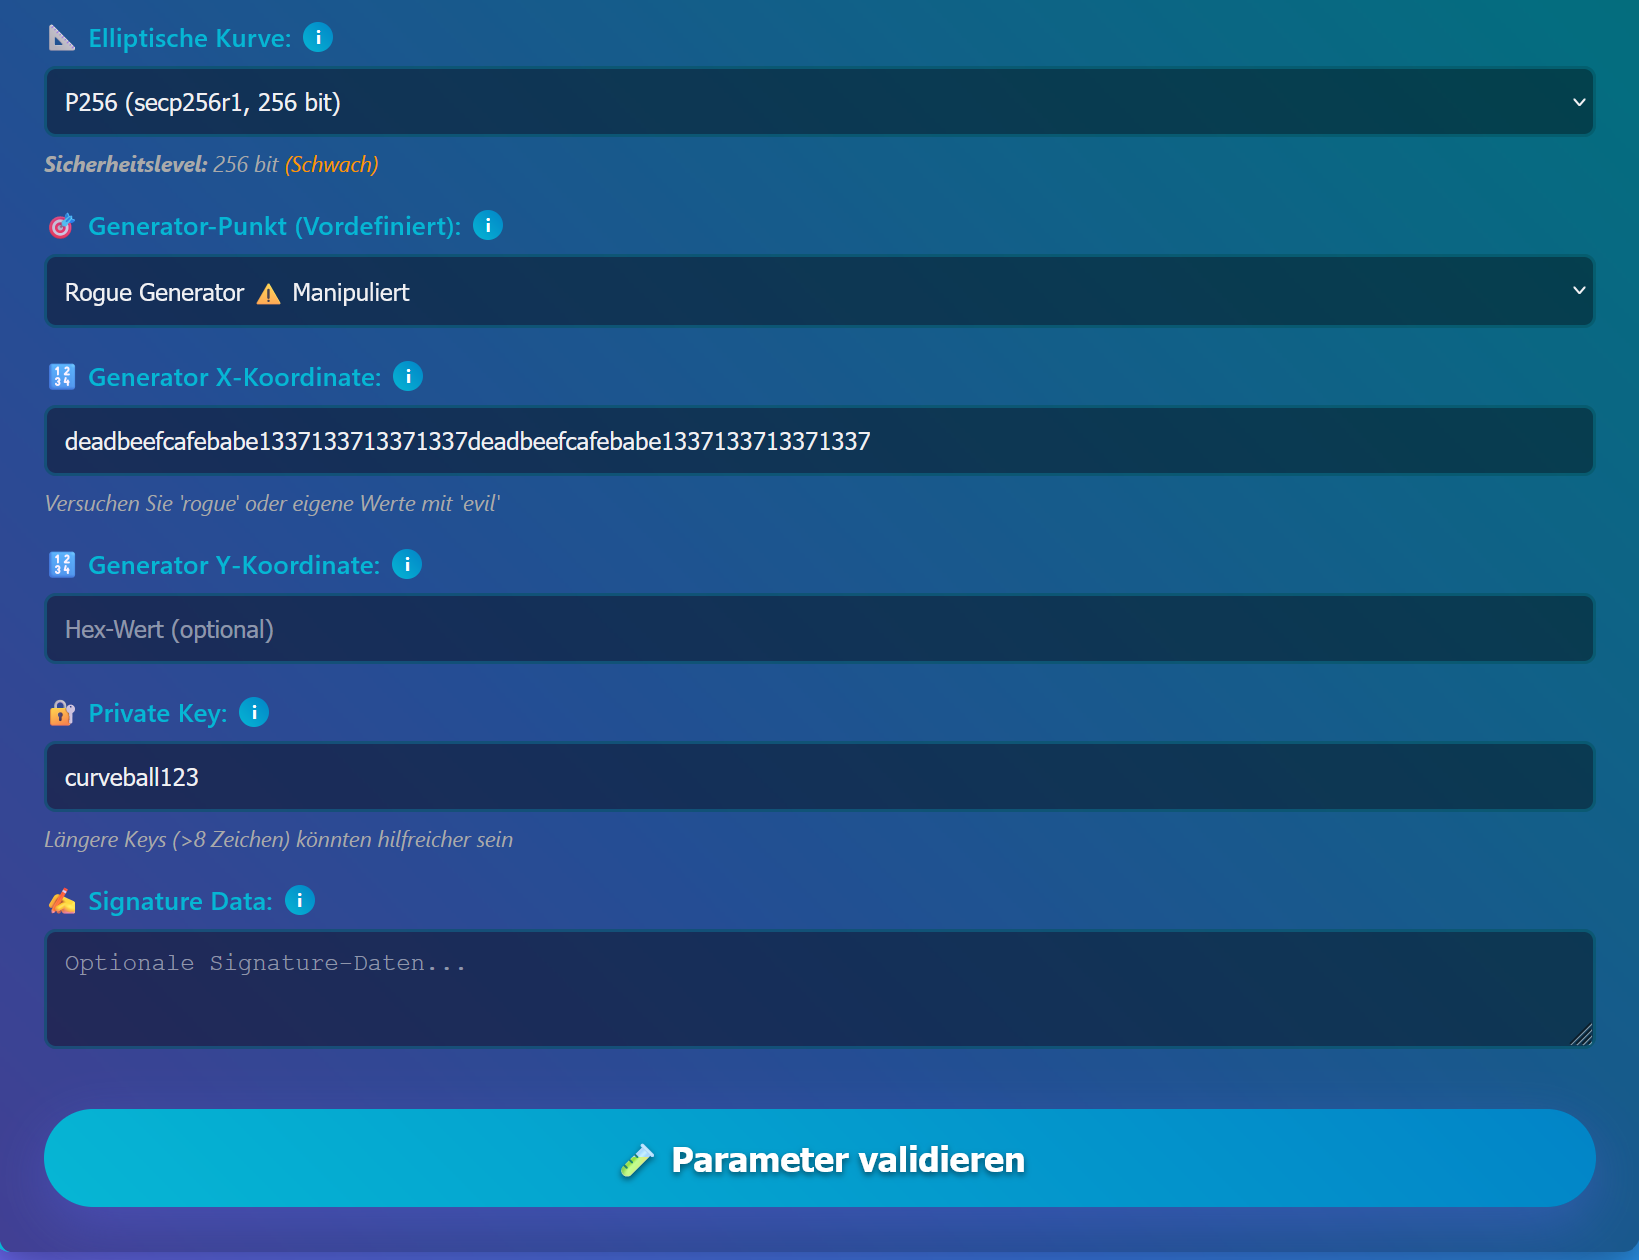
\includegraphics[width=0.8\textwidth]{webinterface_certgen.png}
\caption{Webinterface Zertifikatsgenerierung (Platzhalter)}
\end{figure}

\subsection{Validierungssimulation}
Abschließend prüft das Webinterface mit \texttt{simulate\_vuln\_check.py}, ob die erstellten Zertifikate von der verwundbaren Implementierung akzeptiert werden.

\begin{lstlisting}[language=python,caption={Simulationsprüfung}]
signature = rogue_key.sign_digest(digest)
if rogue_pub.verify_digest(signature, digest):
    print("Vulnerable validation: Signature accepted.")
\end{lstlisting}

\begin{figure}[h]
\centering

\includegraphics[width=0.8\textwidth]{webinterface_validation.png}
\caption{Validierungsergebnis über das Webinterface}
\end{figure}

\section{Technische Hintergründe der Schwachstelle}
Durch gezielte Manipulation des ECC-Generatorpunkts ($G'$) kann ein Angreifer einen privaten Schlüssel erzeugen, der vermeintlich korrekte Signaturen liefert. Windows CryptoAPI validierte die Herkunft des Schlüssels von $G$ nicht, was die Attacke ermöglicht.

\section{Ergebnisse der Simulation}
Die Web-basierte Simulation bestätigte eindrucksvoll, wie einfach manipulierte Zertifikate erzeugt und validiert werden konnten. Die erfolgreiche Validierung im simulierten Szenario zeigt die Gefahr solcher unzureichenden Validierungen.

\section{Fazit}
Das Projekt bietet eine didaktisch wertvolle Möglichkeit, die CurveBall-Schwachstelle praxisnah nachzuvollziehen. Die Webschnittstelle vereinfacht den Lernprozess und verdeutlicht eindrücklich die Gefahren der Schwachstelle.

\newpage

\section*{Eigenständigkeitserklärung}
Hiermit bestätigen wir, dass wir die vorliegende Arbeit selbstständig verfasst und keine anderen Publikationen, Vorlagen und Hilfsmittel als die angegebenen benutzt haben. Alle Teile unserer Arbeit, die wortwörtlich oder dem Sinn nach anderen Werken entnommen sind, wurden unter Angabe der Quelle kenntlich gemacht.

\vspace{1cm}
Deggendorf, \underline{\hspace{0.715\textwidth}}\\
\begin{tabular}{lll}
  \hspace{3cm} & \small(Datum)\hspace{1cm} & \hspace{2cm}\small(Unterschrift)
\end{tabular}
\newpage

\end{document}
